\subsection{Demonstração no simulador}
\label{sec:demo_sim}

Para demonstrar o movimento \textit{move end-effector to target position} para diferentes posições alvo, o manipulador foi levado, no CoppeliaSim, até cada uma das peças detetadas pela câmara na mesa. Para cada alvo, a \texttt{inverse\_kin} calcula os ângulos das juntas, a \texttt{move\_joints} leva o braço até por cima da peça e a \texttt{move\_linear} desce na vertical até 2~cm acima da mesa. Mediram-se três erros:

\begin{itemize}
    \item \textbf{modelo}: distância entre a posição dada pela \texttt{direct\_kin}, com as juntas lidas, e a posição real do centro de preensão no simulador;
    \item \textbf{alcance}: distância entre o ponto pedido e a posição real do centro de preensão;
    \item \textbf{juntas}: maior diferença entre os ângulos calculados e os ângulos lidos.
\end{itemize}

\begin{table}[H]
  \centering
  \caption{Resultados do movimento até diferentes posições alvo no simulador.}
  \label{tab:demo_sim}
  \resizebox{\textwidth}{!}{%
  \begin{tabular}{lcccccc}
    \toprule
    Peça & Pedido $(x, y, z)$ & Alcançado $(x, y, z)$ & $\psi$ & Modelo [mm] & Alcance [mm] & Juntas \\
    \midrule
    vermelho 1 & $(66{,}1;\ 199{,}9;\ -10{,}0)$ & $(65{,}7;\ 196{,}7;\ -11{,}3)$ & $90^\circ$ & 1,5 & 3,5 & $0{,}8^\circ$ \\
    vermelho 2 & $(-111{,}0;\ -37{,}2;\ -10{,}0)$ & $(-111{,}0;\ -38{,}2;\ -10{,}7)$ & $110^\circ$ & 2,3 & 1,3 & $0{,}4^\circ$ \\
    laranja & $(-107{,}9;\ 224{,}1;\ -10{,}0)$ & $(-106{,}0;\ 221{,}2;\ -12{,}4)$ & $90^\circ$ & 2,3 & 4,2 & $1{,}2^\circ$ \\
    amarelo & $(-33{,}5;\ 149{,}7;\ -10{,}0)$ & $(-33{,}0;\ 148{,}0;\ -9{,}7)$ & $95^\circ$ & 1,2 & 1,8 & $0{,}6^\circ$ \\
    verde & $(-129{,}4;\ 54{,}3;\ -10{,}0)$ & $(-128{,}7;\ 53{,}9;\ -10{,}0)$ & $100^\circ$ & 1,2 & 0,8 & $0{,}5^\circ$ \\
    azul & $(-147{,}3;\ 33{,}2;\ -10{,}0)$ & $(-145{,}6;\ 33{,}0;\ -9{,}8)$ & $95^\circ$ & 1,2 & 1,7 & $0{,}6^\circ$ \\
    rosa & $(16{,}3;\ 274{,}4;\ -10{,}0)$ & $(16{,}7;\ 269{,}6;\ -13{,}5)$ & $80^\circ$ & 4,0 & 5,9 & $1{,}6^\circ$ \\
    \bottomrule
  \end{tabular}}
\end{table}

\begin{figure}[H]
  \centering
  \begin{minipage}[b]{0.48\textwidth}
    \centering
    % Peças da demonstração vistas de cima, no referencial da base (cm)
% Zonas iguais às desenhadas na mesa por drawing.draw_zones (mapa calculado
% com plan_vertical + arm_collision):
%   vermelho : junto à base, onde o braço não chega (R_MIN_DIR, 8,4 a 13 cm)
%   azuis    : entre 15,8 e 25,5 cm a garra desce na vertical
%   verde    : 35,2 cm, alcance máximo
%   cunha    : zona morta de J1 (+-165 graus), atrás do robô
% Feita para meia largura de página, sem \resizebox
\begin{tikzpicture}[scale=0.088, >=stealth, every node/.style={font=\scriptsize}]
  \begin{scope}
    \clip (-40,-40) rectangle (40,40);
    \fill[green!8] (0,0) circle (35.2);
    \fill[green!25, even odd rule] (0,0) circle (25.5) (0,0) circle (15.8);
    \draw[green!60!black, line width=0.9pt] (0,0) circle (35.2);
    \draw[blue!80!black, line width=0.9pt] (0,0) circle (25.5);
    \draw[blue!40, line width=0.9pt] (0,0) circle (15.8);
    \filldraw[fill=red!35, draw=red!60!black, line width=0.5pt] (-7.63,-3.51) -- (-8.01,-4.92) -- (-8.35,-6.20) -- (-8.67,-7.40) -- (-8.98,-8.55) -- (-9.28,-9.67) -- (-9.57,-10.76) -- (-9.86,-11.83) -- (-10.14,-12.89) -- (-10.42,-13.93) -- (-10.70,-14.97) -- (-10.97,-16.00) -- (-11.25,-17.02) -- (-11.52,-18.03) -- (-11.79,-19.05) -- (-12.06,-20.05) -- (-12.33,-21.06) -- (-12.60,-22.06) -- (-12.86,-23.05) -- (-13.13,-24.05) -- (-13.40,-25.04) -- (-13.66,-26.03) -- (-13.93,-27.02) -- (-14.19,-28.01) -- (-14.46,-29.00) -- (-14.72,-29.98) -- (-14.98,-30.96) -- (-15.20,-31.75) -- (2.72,-35.10) -- (2.51,-34.31) -- (2.24,-33.32) -- (1.98,-32.34) -- (1.71,-31.35) -- (1.45,-30.37) -- (1.18,-29.38) -- (0.92,-28.39) -- (0.65,-27.39) -- (0.39,-26.40) -- (0.12,-25.40) -- (-0.15,-24.40) -- (-0.42,-23.40) -- (-0.69,-22.39) -- (-0.96,-21.38) -- (-1.23,-20.36) -- (-1.51,-19.34) -- (-1.78,-18.31) -- (-2.06,-17.28) -- (-2.34,-16.23) -- (-2.62,-15.18) -- (-2.91,-14.10) -- (-3.20,-13.01) -- (-3.50,-11.90) -- (-3.81,-10.74) -- (-4.13,-9.54) -- (-4.47,-8.27) -- (-4.85,-6.86) -- cycle;
    \filldraw[fill=red!45, draw=red!60!black, line width=0.6pt] (8.40,0.00) -- (8.37,0.73) -- (8.37,1.48) -- (8.50,2.28) -- (8.55,3.11) -- (8.61,4.01) -- (8.75,5.05) -- (8.76,6.14) -- (8.81,7.39) -- (8.91,8.91) -- (8.36,9.96) -- (7.23,10.32) -- (5.95,10.31) -- (4.82,10.33) -- (3.76,10.34) -- (2.77,10.34) -- (1.82,10.34) -- (0.91,10.36) -- (0.00,10.40) -- (-0.91,10.36) -- (-1.82,10.34) -- (-2.77,10.34) -- (-3.76,10.34) -- (-4.86,10.42) -- (-6.05,10.48) -- (-7.40,10.57) -- (-8.36,9.96) -- (-8.34,8.34) -- (-8.35,7.01) -- (-8.36,5.85) -- (-8.31,4.80) -- (-8.34,3.89) -- (-8.36,3.04) -- (-8.31,2.23) -- (-8.37,1.48) -- (-8.37,0.73) -- (-8.40,0.00) -- (-8.37,-0.73) -- (-8.37,-1.48) -- (-8.50,-2.28) -- (-8.55,-3.11) -- (-8.61,-4.01) -- (-8.75,-5.05) -- (-8.76,-6.14) -- (-8.81,-7.39) -- (-8.91,-8.91) -- (-8.36,-9.96) -- (-7.23,-10.32) -- (-5.95,-10.31) -- (-4.82,-10.33) -- (-3.76,-10.34) -- (-2.77,-10.34) -- (-1.82,-10.34) -- (-0.91,-10.36) -- (-0.00,-10.40) -- (0.91,-10.36) -- (1.82,-10.34) -- (2.77,-10.34) -- (3.76,-10.34) -- (4.86,-10.42) -- (6.05,-10.48) -- (7.40,-10.57) -- (8.36,-9.96) -- (8.34,-8.34) -- (8.35,-7.01) -- (8.36,-5.85) -- (8.31,-4.80) -- (8.34,-3.89) -- (8.36,-3.04) -- (8.31,-2.23) -- (8.37,-1.48) -- (8.37,-0.73) -- cycle;
  \end{scope}
  % eixos
  \draw[->, thin] (-39,0) -- (41,0) node[below left=0pt and -2pt] {$x$};
  \draw[->, thin] (0,-39) -- (0,41) node[left] {$y$};
  \fill[gray!60] (0,0) circle (1.5);
  % raios
  \node[blue!50!black, fill=white, inner sep=0.5pt, font=\tiny] at (20:15.8) {15,8};
  \node[blue!70!black, fill=white, inner sep=0.5pt, font=\tiny] at (20:25.5) {25,5};
  \node[green!35!black, fill=white, inner sep=0.5pt, font=\tiny] at (20:35.2) {35,2};
  % peças alcançadas
  \foreach \x/\y/\c/\n/\p in {
      6.61/19.99/red!75!black/vermelho 1/right,
      -11.10/-3.72/red!75!black/vermelho 2/below left,
      -10.84/22.46/orange!90!black/laranja/left,
      -3.35/14.97/yellow!70!black/amarelo/right,
      -12.94/5.43/green!50!black/verde/above,
      -14.73/3.32/blue!70!black/azul/left,
      1.63/27.49/magenta!80!black/rosa/right} {
    \filldraw[fill=\c, draw=black, thin] (\x,\y) circle (1.3);
    \node[\p=1pt, inner sep=1pt] at (\x,\y) {\n};
  }
  % legenda
  \begin{scope}[shift={(-39,-45)}]
    \filldraw[fill=green!25, draw=green!50!black] (0,-2.5) rectangle (3,0.5);
    \node[right] at (3.5,-1) {garra vertical};
    \filldraw[fill=green!8, draw=green!50!black] (35,-2.5) rectangle (38,0.5);
    \node[right] at (38.5,-1) {garra inclinada};
    \filldraw[fill=red!45, draw=red!60!black] (0,-8.5) rectangle (3,-5.5);
    \node[right] at (3.5,-7) {sem alcance};
    \draw[green!60!black, line width=0.9pt] (35,-7) -- (38,-7);
    \node[right] at (38.5,-7) {alcance máximo};
  \end{scope}
\end{tikzpicture}
    \caption{Peças da demonstração vistas de cima, no referencial da base (cm), com os limites de alcance.}
    \label{fig:mapa_alvos}
  \end{minipage}\hfill
  \begin{minipage}[b]{0.48\textwidth}
    \centering
    % Erros de modelo e de alcance, ordenados pela distância ao eixo da base (precisa de \usepackage{pgfplots})
% Feita para meia largura de página (dentro de uma minipage de 0,48\textwidth), sem \resizebox
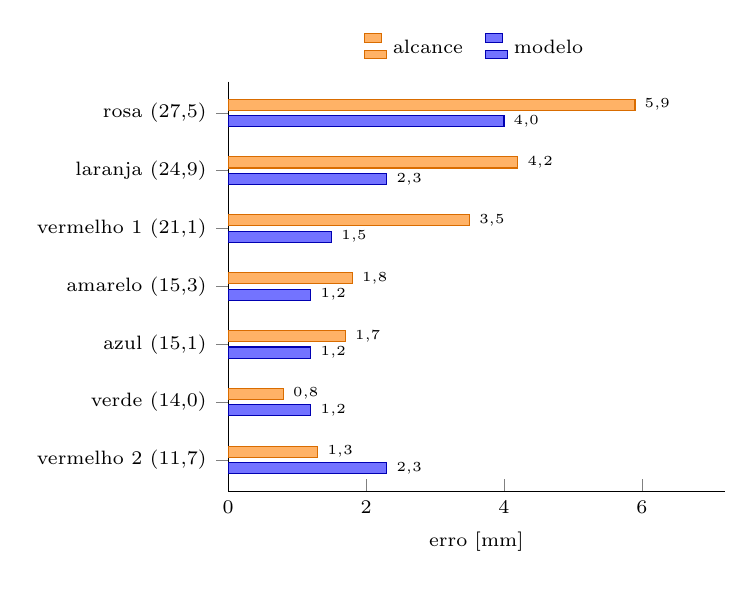
\begin{tikzpicture}
  \begin{axis}[xbar, bar width=4pt, scale only axis, width=0.52\linewidth, height=5.2cm,
      xmin=0, xmax=7.2, xlabel={erro [mm]},
      symbolic y coords={rosa, laranja, vermelho 1, amarelo, azul, verde, vermelho 2},
      ytick=data,
      yticklabels={{rosa (27,5)}, {laranja (24,9)}, {vermelho 1 (21,1)}, {amarelo (15,3)}, {azul (15,1)}, {verde (14,0)}, {vermelho 2 (11,7)}},
      y dir=reverse, enlarge y limits=0.09,
      tick label style={font=\scriptsize}, label style={font=\scriptsize},
      nodes near coords, every node near coord/.append style={font=\tiny},
      /pgf/number format/use comma, /pgf/number format/fixed, /pgf/number format/precision=1,
      /pgf/number format/fixed zerofill,
      legend style={at={(0.5,1.03)}, anchor=south, font=\scriptsize, draw=none, fill=none, legend columns=2, /tikz/every even column/.append style={column sep=6pt}},
      reverse legend,
      legend cell align=left,
      axis lines*=left, xtick={0,2,4,6}, xticklabels={0,2,4,6}]
    \addplot[fill=blue!55, draw=blue!70!black] coordinates
      {(4.0,rosa) (2.3,laranja) (1.5,vermelho 1) (1.2,amarelo) (1.2,azul) (1.2,verde) (2.3,vermelho 2)};
    \addplot[fill=orange!60, draw=orange!85!black] coordinates
      {(5.9,rosa) (4.2,laranja) (3.5,vermelho 1) (1.8,amarelo) (1.7,azul) (0.8,verde) (1.3,vermelho 2)};
    \legend{modelo, alcance}
  \end{axis}
\end{tikzpicture}
    \caption{Erros de modelo e de alcance em cada peça.}
    \label{fig:erros}
  \end{minipage}
\end{figure}

Nos sete alvos alcançáveis, a garra chegou a menos de 6~mm do ponto pedido e as juntas ficaram a menos de $1{,}6^\circ$ dos ângulos calculados. A altura $z = -10$~mm no referencial da base corresponde a 20~mm acima da mesa. Quatro peças, a 39--41~cm do eixo da base, foram declaradas inalcançáveis pela cinemática inversa antes de o braço se mover. O erro de alcance cresce com a distância ao eixo da base, sendo máximo no alvo mais afastado (rosa, a 27~cm), o que é compatível com o braço a descair com o próprio peso quando está mais esticado.